\PassOptionsToPackage{x11names}{xcolor}
\documentclass[14pt,aspectratio=169,xcolor=dvipsnames]{beamer}
\usetheme{SimplePlus}

%%%% used for timeline
\usepackage{colortbl}
\usepackage{caption}
\usepackage{booktabs}
\DeclareCaptionFont{blue}{\color{LightSteelBlue3}}
\newcommand{\foo}{\color{LightSteelBlue3}\makebox[0pt]{\textbullet}\hskip-0.5pt\vrule width 1pt\hspace{\labelsep}}

%%%%%%%%%%%%%%%%%%%%%%%%%%%%%

\title[short title]{Clase 1: Introducción a la programación}
\subtitle{}
\author[NA Barnafi] {Nicolás Alejandro Barnafi Wittwer}
\institute[UC|CMM] 
{
    Pontificia Universidad Católica de Chile \\
    Centro de Modelamiento Matemático
}

\titlegraphic{
    \vspace{-1.8cm}
    \begin{flushright}
      
\includegraphics[height=2.5cm]{../images/logos/puc.png} 
    \end{flushright}
}

\date{07/08/2024}


\begin{document}
%%%%%%%%%%%%%%%%%%%%%%%%%%%%%%%%%%%%%%%%%%%%%%%%%%%%%%%
\begin{frame}
    \maketitle
\end{frame}
%%%%%%%%%%%%%%%%%%%%%%%%%%%%%%%%%%%%%%%%%%%%%%%%%%%%%%%
\section{Introducción a la programación}
%%%%%%%%%%%%%%%%%%%%%%%%%%%%%%%%%%%%%%%%%%%%%%%%%%%%%%%
\begin{frame}[t]\frametitle{Qué es programar}
  \idea{ Hacer que el computador haga algo a partir de instrucciones}

\begin{itemize}
    \item Instrucciones: \emph{lenguaje de programación}
    \item Ejs: 
        \begin{itemize}
            \item Web (HTML,CSS,PHP,JS)
            \item Apps (Java)
            \item {\only<2>{\bf\color{MediumGreen}}Ciencia (Python,R,Julia,MATLAB)}
            \item Esta presentación (\LaTeX)
        \end{itemize}
\end{itemize}

\vspace{1cm}
\pause \alertGreen{El foco del curso estará en programación científica}
\end{frame}
%%%%%%%%%%%%%%%%%%%%%%%%%%%%%%%%%%%%%%%%%%%%%%%%%%%%%%%
\begin{frame}\frametitle{Lecturas muy recomendadas}
\texttt{https://swcarpentry.github.io/python-novice-inflammation/}

\texttt{https://rosalind.info}
\end{frame}
%%%%%%%%%%%%%%%%%%%%%%%%%%%%%%%%%%%%%%%%%%%%%%%%%%%%%%%
\begin{frame}[t]\frametitle{Ejemplo: Artritis}
Imaginen que tenemos una cura milagrosa para la artritis que actúa en 3 semanas. 
\begin{itemize}
    \item<1-> Seguimiento pacientes: Dosis después de primer síntoma
    \item<2-> Datos: Nro de inflamaciones por día
        \only<2>{
            \begin{flushright}
                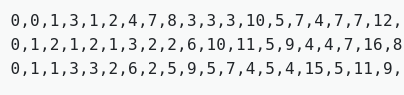
\includegraphics[width=0.5\textwidth]{../images/datos-artritis.png}
            \end{flushright}
        }
    \item<3-> Visualización
        \only<3>{
            \begin{flushright}
                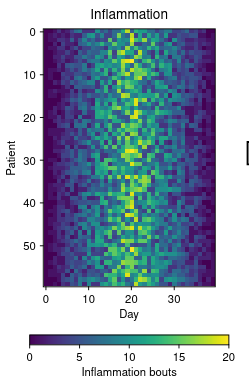
\includegraphics[width=0.3\textwidth]{../images/datos-artritis2.png}
            \end{flushright}
        }
    \item<4-> Concluir!
\end{itemize}
\end{frame}
%%%%%%%%%%%%%%%%%%%%%%%%%%%%%%%%%%%%%%%%%%%%%%%%%%%%%%%
\begin{frame}\frametitle{Ej II: Pensamiento algorítmico}
Cómo salgo de esta sala? 

\vspace{2cm}
\pause Y si solo se girar a la derecha?

\end{frame}
%%%%%%%%%%%%%%%%%%%%%%%%%%%%%%%%%%%%%%%%%%%%%%%%%%%%%%%
\begin{frame}\frametitle{Ej II: Lo que hicimos}
    \begin{itemize}
        \item Considerar un pequeño conjunto de instrucciones
        \item Generar nuevas instrucciones más complejas {\color{gray}(como la célula!)}
        \item Combinar instrucciones para un objetivo
    \end{itemize}
\end{frame}
%%%%%%%%%%%%%%%%%%%%%%%%%%%%%%%%%%%%%%%%%%%%%%%%%%%%%%%
\section{Interacción con el PC}
%%%%%%%%%%%%%%%%%%%%%%%%%%%%%%%%%%%%%%%%%%%%%%%%%%%%%%%
\begin{frame}\frametitle{Sistemas operativos}
El OS coordina funcionamiento del computador. \pause
    \begin{itemize}
        \item<+-> Windows (MS-DOS)
        \item<+-> Mac OS (BSD Darwin)
        \item<+-> BSD (FreeBSD, OpenBSD)
        \item<+-> GNU/Linux (Debian, Ubuntu, Fedora, $\hdots$)
        \item<+-> Android
        \item<+-> iOS
        \item<+-> Symbian
        \item<+-> BeOS, Haiku
    \end{itemize}
\end{frame}
%%%%%%%%%%%%%%%%%%%%%%%%%%%%%%%%%%%%%%%%%%%%%%%%%%%%%%%
\begin{frame}\frametitle{Sistemas operativos}
    \begin{center}
        %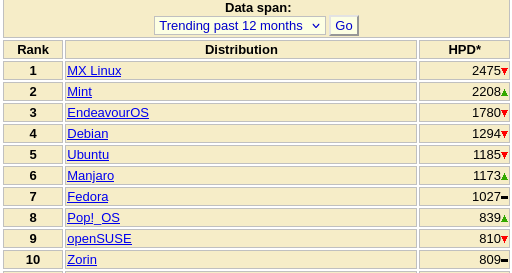
\includegraphics[width=0.5\textwidth]{../images/distrowatch.png}
    \end{center}
\end{frame}
%%%%%%%%%%%%%%%%%%%%%%%%%%%%%%%%%%%%%%%%%%%%%%%%%%%%%%%
\begin{frame}\frametitle{Sistemas operativos}
    \begin{columns}
        \begin{column}{0.45\textwidth}
        \begin{small}
        \begin{table}
            \renewcommand\arraystretch{1.4}\arrayrulecolor{LightSteelBlue3}
            %\captionsetup{singlelinecheck=false, font=blue, labelfont=sc, labelsep=quad}

            %\begin{minipage}{7cm}
                %\caption*{}
            %\end{minipage}
            \vskip -1.5ex

            \begin{tabular}{@{\,}r <{\hskip 2pt} !{\foo} >{\raggedright\arraybackslash}p{5cm}}
            \addlinespace[1.5ex]
            1956   & General Motors  \\
            1960's & UNIX  \\
            1977   & Apple \\
            1981   & MS-DOS \\
            1991   & Linux (GNU/Linux) \\
            1995   & Windows 95 \\
            2000   & Darwin (macOS) \\
            2007   & iOS \\
            2008   & Android
            \end{tabular}
        \end{table}
        \end{small}
        \end{column}
        \begin{column}{0.5\textwidth}
            \only<1>{
                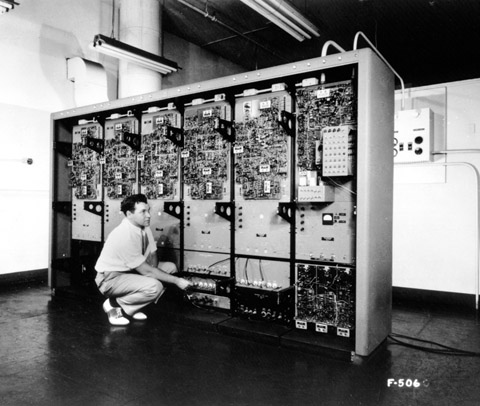
\includegraphics[width=\textwidth]{../images/os-gm.png}
                GM para primer IBM }
            \only<2>{
                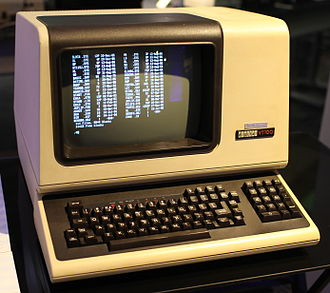
\includegraphics[width=0.9\textwidth]{../images/os-unix.png}
                Terminal UNIX}
            \only<3>{
                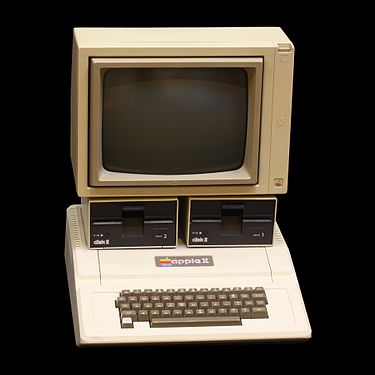
\includegraphics[width=0.8\textwidth]{../images/os-appleii.png}
                Primer Apple ][}
            \only<4>{
                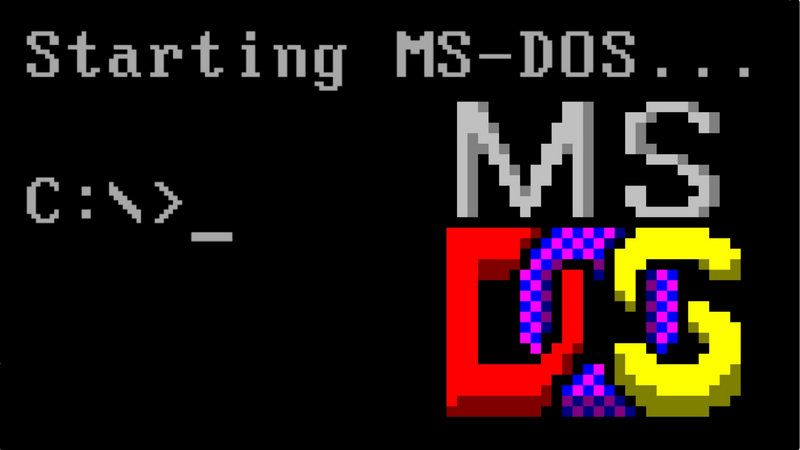
\includegraphics[width=\textwidth]{../images/os-msdos.png}
                MSDOS (Microsoft)}
            \only<5>{
                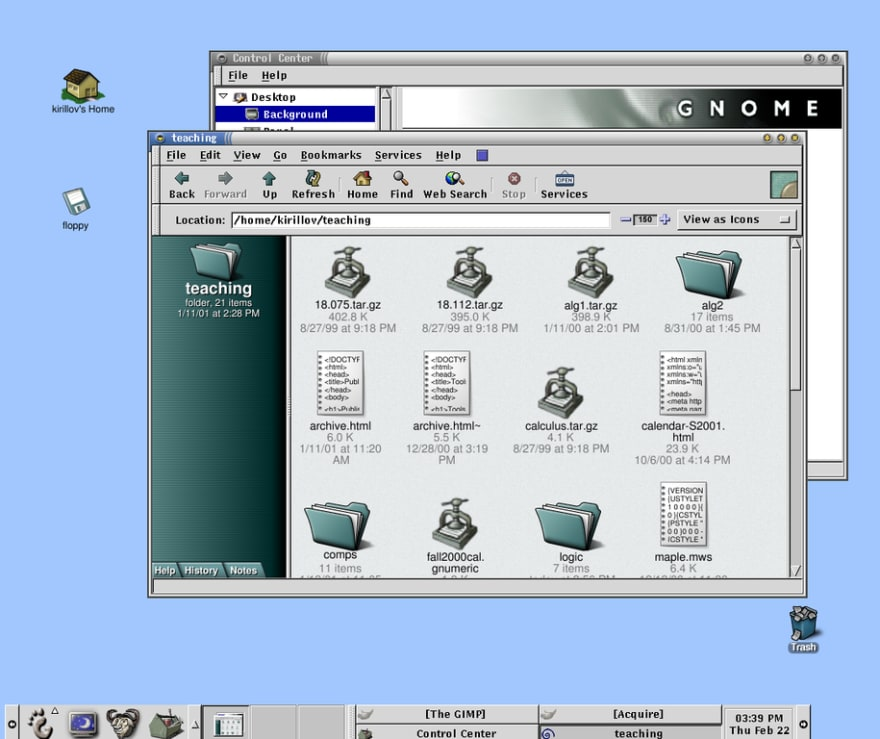
\includegraphics[width=\textwidth]{../images/os-linux.png}
                Linux desktop}
            \only<6>{
                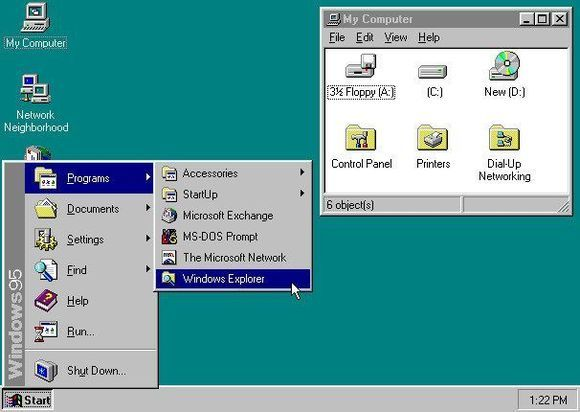
\includegraphics[width=\textwidth]{../images/os-windows95.png}
                Escritorio \emph{moderno} (Win95) }
            \only<7>{
                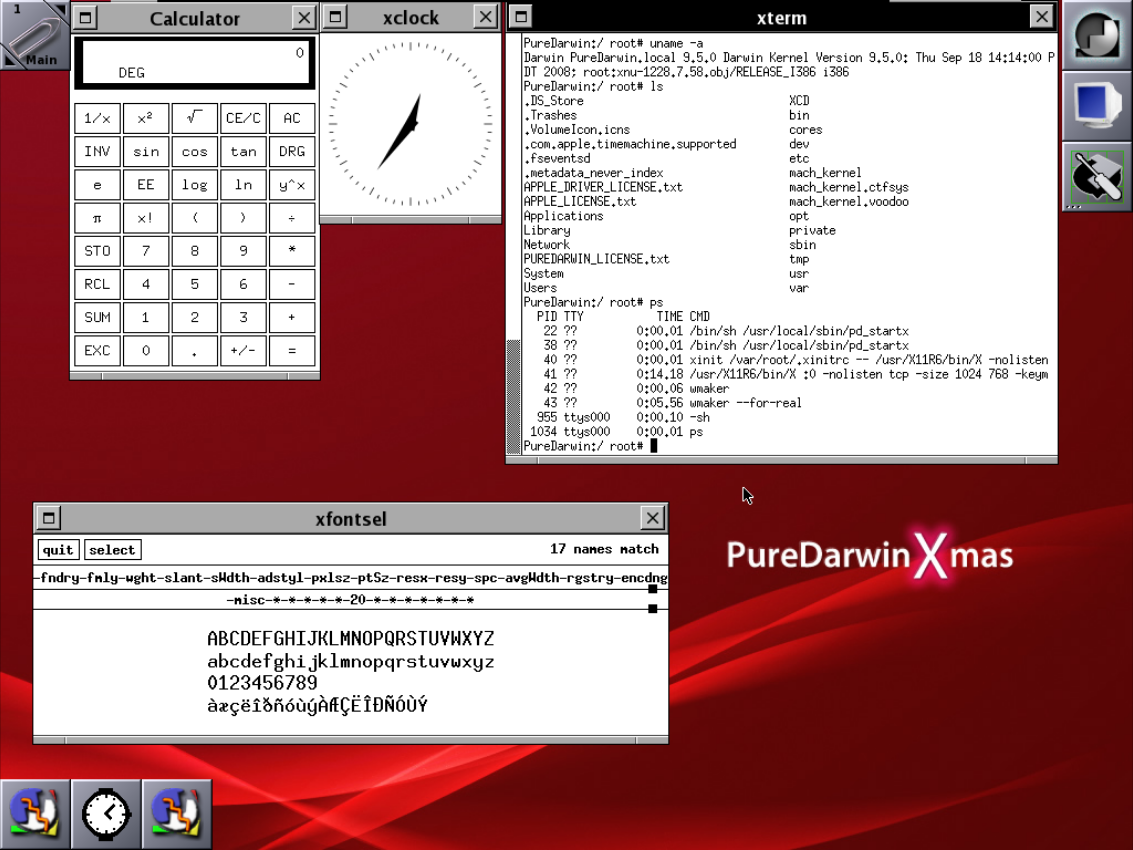
\includegraphics[width=\textwidth]{../images/os-darwin.png}
                Bases de macOS}
            \only<8>{
                
\includegraphics[width=\textwidth]{../images/os-ios.png}
                }
            \only<9>{
                
\includegraphics[width=0.8\textwidth]{../images/os-android.png}
                }
        \end{column}
    \end{columns}
\end{frame}
%%%%%%%%%%%%%%%%%%%%%%%%%%%%%%%%%%%%%%%%%%%%%%%%%%%%%%%
\begin{frame}\frametitle{Recap}
    \begin{itemize}
        \item Qué es programar
        \item Pensamiento algorítmico
        \item Sistemas operativos
    \end{itemize}
\end{frame}
%%%%%%%%%%%%%%%%%%%%%%%%%%%%%%%%%%%%%%%%%%%%%%%%%%%%%%%
\begin{frame}
    \maketitle
\end{frame}
%%%%%%%%%%%%%%%%%%%%%%%%%%%%%%%%%%%%%%%%%%%%%%%%%%%%%%%

\end{document}
